% siehe auch Abb. 13.5 auf S. 211 aus „Atom- und Quantenphysik“ von Haken/Wolf 1990

% \documentclass[tikz]{standalone}

% https://tex.stackexchange.com/a/36607
\newcommand{\AxisRotator}[1][rotate=0]{%
    \tikz [x=5,y=10,-stealth,#1] \draw (0,0) arc (-150:150:1 and 1);%
}

% \begin{document}
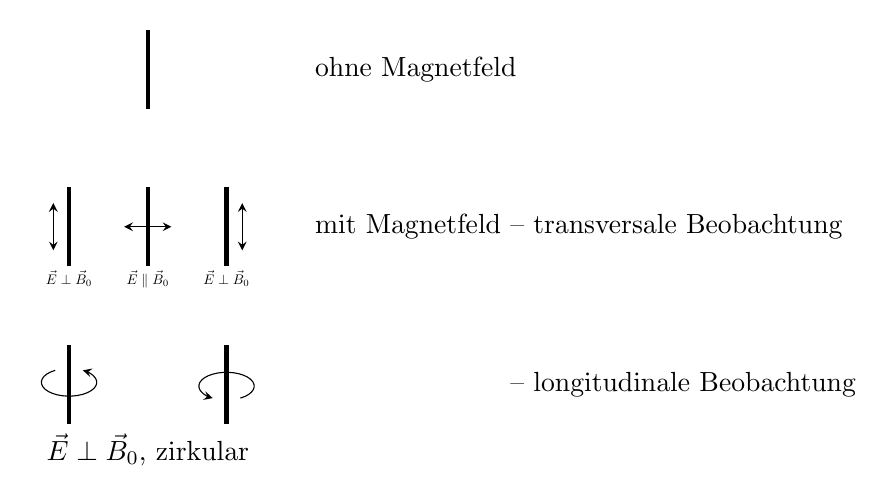
\begin{tikzpicture}
    \draw[ultra thick] (0,+2) -- (0,+3);

    \draw[ultra thick] (-1,0) -- (-1,+1);
    \draw[stealth-stealth](-1.2,0.2) -- (-1.2,0.8);
    \node[scale=0.5, anchor=north] at (-1,0) {$\vec E \perp \vec B_0$};
    \draw[ultra thick] (0,0) -- (0,+1);
    \draw[stealth-stealth](-0.3,0.5) -- (+0.3,0.5);
    \node[scale=0.5, anchor=north] at (0,0) {$\vec E \parallel \vec B_0$};
    \draw[ultra thick] (+1,0) -- (+1,+1);
    \draw[stealth-stealth](+1.2,0.2) -- (+1.2,0.8);
    \node[scale=0.5, anchor=north] at (+1,0) {$\vec E \perp \vec B_0$};

    \draw[ultra thick] (-1,-2) -- (-1,-1) node [midway] {\AxisRotator[rotate=270]};
    \draw[ultra thick] (+1,-2) -- (+1,-1) node [midway] {\AxisRotator[rotate=90]};
    \node[anchor=north] at (0,-2) {$\vec E \perp \vec B_0$, zirkular};

    \node[anchor=west] at (2,2.5) {ohne Magnetfeld};
    \node[anchor=west] at (2,0.5) {mit Magnetfeld – transversale Beobachtung};
    \node[anchor=west] at (2,-1.5) {\phantom{mit Magnetfeld} – longitudinale Beobachtung};
\end{tikzpicture}
% \end{document}
